\section{Proposed Approach: Effective Partnerships Adjustment}\label{foi.prop}
An approach to modelling HIV transmission via sexual partnerships
that addresses the above limitations
while remaining within the traditional compartmental framework would be useful.
In this section, we develop and propose such an approach:
the \emph{Effective Partnerships Adjustment} (EPA).%
\footnote{A preliminary version of this approach was presented in \cite{Knight2022smdm}.}
That is, this approach overcomes
the main limitations of prior approaches described above,
without changing to a pair-based or individual-based modelling framework \cite{Rao2021}.
%===================================================================================================
\subsection{Conceptual Development}\label{foi.prop.concept}
% SM: LOVE this section
% JK: thanks!
A core challenge of modelling HIV transmission via sexual partnerships is
to account for inert sex acts.
Any partnership where transmission has already occurred
is seroconcordant and thus ``transmission ineffective'',
and so should be removed from the force of infection.%
\footnote{An illustrative scenario to highlight this issue is given in \sref{sr.foi.toy}.}
Our fundamental insights is that:
in a compartmental (non-pair-based) model,
these partnerships can be tracked as proportions of individuals, namely:
all individuals who recently acquired infection \emph{and}
all individuals who recently transmitted infection.
Here, we use ``recently'' to mean ``before individuals change partners''.
If some individuals have multiple concurrent partners,
then these individuals should not be removed entirely,
but their numbers of ``effective partnerships'' should be reduced by 1.
If multiple types of partnerships are considered,
then only the partnership type involved in the transmission should be reduced.
This adjustment to ``effective partnerships'' can then be applied
until these individuals change partners
% TODO: (*) but part of partnership has already passed, so delta_new < delta_total
--- at a rate inversely related to the partnership duration: $\delta^{-1}$.
However, during this period, these individuals can/should still be modelled
to progress as usual through different stages of infection, treatment, etc.
\par
Using this conceptual basis,
we propose a new stratification of the modelled infected population, denoted $\p$.
The stratum $\p = 0$ corresponds to no recent transmission,
or all ``new'' (potentially serodiscordant) partnerships.
Other strata $\p > 0$ correspond to recent transmission via (to or from) partnership type $\p$.
Figure~\ref{fig:model.hiv.p} illustrates the new stratification
together with with an existing HIV infection stratification (Figure~\ref{fig:model.hiv}).
Following infection, all individuals enter a stratum $\p > 0$
corresponding to the partnership type $p$ by which they were infected.
Thus, the rate of entry to this stratum among susceptibles is defined by
the force of infection without aggregating across partnership types: $\lambda_{p}$.
Individuals may then transition from $\p > 0$ to $\p = 0$
upon forming a new partnership, at a rate $\delta_p^{-1}$.
Finally, individuals may re-enter any stratum $\p > 0$
if they transmit infection via partnership type $p$.
We denote the corresponding rate as $\lambda'_{p}$,
representing the per-person rate of \emph{transmission},
not \emph{acquisition} as in $\lambda_{p}$.
This rate $\lambda'_{p}$ is not defined or needed in prior approaches (\sref{foi.prior})
but we develop the necessary equations below in \sref{foi.prop.eq}.
The issue of multiple concurrent post-transmission partnerships is discussed in \sref{foi.prop.mp}.
\begin{figure}
  \centering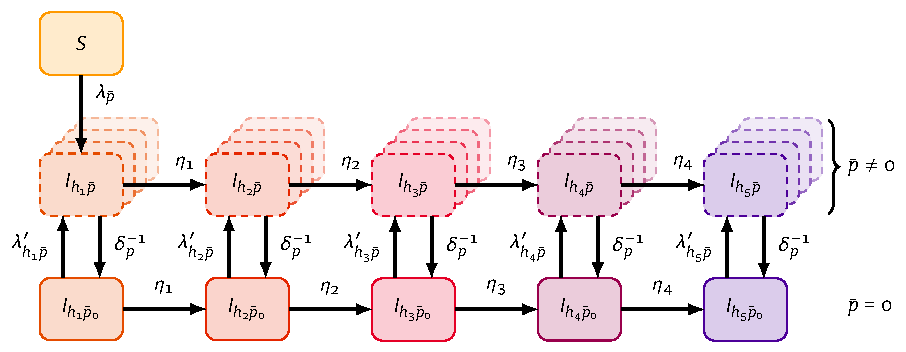
\includegraphics[scale=1]{model.hiv.p}
  \caption{Modelled states and transitions related to HIV infection,
    and a new stratification $\p$ to track
    the proportions of individuals in partnerships where transmission already occurred}
  \label{fig:model.hiv.p}
  \floatfoot{
    $S$: susceptible;
    $I_{h}$: infectious in stage $h$;
    $p$: partnership type;
    $\p$: new stratification, where
      $\p = 0$ reflects no recent transmission (all new partnerships), and
      $\p > 0$ reflects recent transmission via a type-$p$ partnership;
    $\lambda$: force of infection per susceptible;
    $\lambda'$: force of infection per infectious;
    $\eta$: rate of progression between infection stages;
    $\delta$: partnership duration.}
\end{figure}
%===================================================================================================
\subsection{Equations}\label{foi.prop.eq}
Since partnership duration is now considered separately and explicitly,
we need not define any per-partnership probability of transmission $B$.
Rather, we define the force of infection to directly include
the frequency of sex per partnership $F$ and probability of transmission per sex act $\beta$.
However, the mixing is slightly more complicated than before,
since the number of ``effective partnerships'' depends on infection status.
In addition, these partnerships are now defined as numbers of current partners~$K$,
rather than rates of partnership formation~$Q$.
\par
Let $M_{pii'}$ be the total (population-level, not per-person)
number of type-$p$ partnerships between risk groups $i$~and~$i'$.
This ``mixing matrix'' $M_{pii'}$ can be defined in several ways (\eg \sref{mod.par.mix}),
based on the total numbers of ``effective partnerships'' among each group: $M_{pi}, M_{pi'}$,
plus some parameter(s) specifying mixing patterns.
Working backwards, we start by defining $M_{pi}$ (and likewise $M_{pi'}$) via
the sum across health statuses --- \ie susceptible and different stages of infection~$h$:
\begin{equation}\label{eq:M.SI}
  M_{pi} = M_{S,pi} + \sum_h M_{I,pih}
\end{equation}
We define the total numbers of partnerships among susceptible individuals as:
\begin{equation}\label{eq:M.S}
  M_{S,pi} = S_{i} K_{pi}
\end{equation}
and likewise for individuals in infection stage $h$ as:
\begin{equation}\label{eq:M.I}
  M_{I,pih} = I_{ih,\p=p} (K_{pi}-1) + \sum\nolimits_{\p \ne p} I_{ih\p}\,K_{pi}
\end{equation}
This \eqref{eq:M.I} is the key equation whereby
the  numbers of ``effective type-$p$ partnerships'' among
individuals in stratum $\p$ are reduced by 1.
This reduction is then propagated through the mixing patterns when defining $M_{pii'}$.
% TODO: (*) double-check that this reduction should be propagated through the mixing patterns
% SM: not sure I follow what this means re: propogated through the mixing patterns?
%     i think we mean the effective reduction is propogated (like herd effects essentially?)
%     but that the actual partnersips are not influenced by whether transmissions occurred or not
%     (i.e. we assume no behavoiur change following transmission?)
% JK: Damn it, you're right :) That is, the current implementation does in fact
%     induce mixing changes due to transmission. I had convinced myself it didn't
%     since mixing is implemented via "log-odds" (Morris) which is "invariant to margins"
%     but this ignores the fact that transmission removes elements from the
%     global current partners matrix M_{pii'} non-randomly.
%     I think it may be a simple fix, so I will try to think more addition
%     update to this section and maybe we can discuss how to proceed.
Next, we define the total (population-level, not per-person) rate of transmission
from group $i'$ and infection stage $h'$ to group $i$ via type-$p$ partnerships as:
\begin{equation}
  \Lambda_{pii'h'} = F_p \beta_{pii'h'} M_{pii'}
  \left(\frac{M_{S,pi}}{M_{pi}}\right)
  \left(\frac{M_{I,pi'h'}}{M_{pi'}}\right)
\end{equation}
where the two fractions represent the proportions of all type-$p$ partnerships $M_{pii'}$
that are formed between susceptible individuals from group $i$ ($M_{S,pi}$)
and infectious individuals in group/infection stage $i'h'$ ($M_{I,pi'h'}$).
The per-person transmission rates to group $i$, and from group $i'h'$
(Figure~\ref{fig:model.hiv.p}) can then be defined as:
\begin{alignat}{1}
  \lambda_{pi} &= \sum_{i'h'} \Lambda_{pii'h'}\,{S_{i}}^{-1} \label{eq:foi.i} \\
  \lambda'_{pi'h'} &= \sum_{i} \Lambda_{pii'h'}\,{I_{i'h'}}^{-1} \label{eq:foi.jh}
\end{alignat}
For the purposes of solving the model,
we can skip division by $S_{i}$ and $I_{i'h'}$ in \eqrefs{eq:foi.i}{eq:foi.jh},
since $\lambda'_{pi}$ and $\lambda'_{pi'h'}$ are immediately multiplied by $S_{i}$ and $I_{i'h'}$,
respectively, in the system of differential equations
--- \ie we need total, not per-person, rates of transmission.
\par
Finally, and to reiterate from above, infected individuals in stratum $I_{ih\p}$
are assumed to form new partnerships at a rate $\delta_p^{-1}$,
and thereby transition to stratum $I_{ih\p_0}$ (``all new partners''); and
otherwise transition between infection stages, cascade of care, activity groups, etc. as usual,
as illustrated in Figure~\ref{fig:model.hiv.p}.
%===================================================================================================
\subsection{Transmission via Multiple Partnerships}\label{foi.prop.mp}
In the proposed EPA approach,
we do not explicitly model the proportions of infected individuals
who recently acquired and/or transmitted infection via
two partnerships of the same type or two different partnership types.
To do so, the required size of the new dimension $\p$ would be at least $2^{P}$, not $P+1$,
where $P$ is the number of different partnership types modelled.
For transmission via three different partnerships,
the required size would be at least $3^{P}$, and so on.
Indeed, this exponential relationship is related to the challenge of specifying
all possible combinations of partnership states in pair-based models \cite{Kretzschmar2017}.
However, under frequentist assumptions, we can equivalently model
two transmissions by one individual as one transmission each by two individuals.
Thus, we can transfer two individuals from $I_{ih\p_0}$ to
$I_{ih\p_1}$ and $I_{ih\p_2}$ (one each) under the proposed $P+1$ stratification,
instead of just one individual from $I_{ih\p_0}$ to
``$I_{ih\p_{12}}$'' under an exponential ($x^P$) stratification.
\par
In fact, $I_{ih\p_0}$ can be \emph{negative} (but only for $\p = 0$),
because the dimension $\p$ is only relevant to \eqref{eq:M.I};
in all other contexts and equations,
we use $I_{ih} = \sum_{\p} I_{ih\p}$, which must be positive as usual.
Moreover, we can also have $I_{ih\p} > I_{ih}$, provided that:
\begin{equation}\label{eq:I.constr}
  I_{ih\p} \le I_{ih} K_{pi}
\end{equation}
reflecting the situation where $>100$\% of $I_{ih}$
have recently acquired and/or transmitted infection via at least one type-$p$ partnership,
or $>50$\% via at least two partnerships, etc.
This situation can therefore only arise in the context of
multiple concurrent type-$p$ partnerships: $K_{pi} > 1$.
If $I_{ih\p} > I_{ih}$, then $I_{ih\p_0}$ \emph{must} be negative,
but we can show that \eqref{eq:M.I} still yields the correct value of $M_{I,pih}$.
With this perspective, the constraint in \eqref{eq:I.constr} may be more intuitive:
we cannot ``remove'' more than the total number of current partnerships.
This constraint should also be easy to guarantee for a small enough timesteps,
because in \eqref{eq:M.I}, $M_{I,pih}$ approaches zero as $I_{ih\p}$ approaches $I_{ih} K_{pi}$
--- i.e. all type-$p$ partnerships become seroconcordant-infected,
and no more transmission can occur via these partnerships until partners change.
%===================================================================================================
\subsection{Transmission-Driven Seroconcordance}\label{foi.prop.tdsc}
Another benefit of the proposed approach is that
we can quantify the proportion of partnerships that are seroconcordant
due to prior transmission within the partnership.
We call these partnerships ``transmission-driven seroconcordant''
to distinguish them from seroconcordant partnerships \emph{newly} formed
by chance or due to serosorting \cite{Purcell2017,Kim2020}
among two previously infected individuals.
For this proportion,
the numerator is the population size of stratum $\p=p$, while
the denominator is the total number of type-$p$ partnerships among
(a) all individuals, or (b) infected individuals only:
\begin{equation}\label{eq:tdsc}
  \textsc{tdsc}_{p*} = \frac{I_{*,\p=p}}{K_{p*} \sum_{\p} X_{*\p}}
  \qquad
  \begin{cases}
    X = I + S & \textnormal{(a)} \\
    X = I     & \textnormal{(b)} \\
  \end{cases}
\end{equation}
where $*$ could specify any subset of the population
defined by modelled strata --- \eg sex, activity group, HIV state, etc.
While denominator (a) may be interesting conceptually,
denominator (b) can be more directly interpreted as
a relative reduction in onward transmission risk among infected individuals
due to infections ``trapped'' within partnerships.
The actual total reduction would be weighted by
the probability of transmission per sex act, sex frequency, etc.
We also note that a single post-transmission partnership
will be ``double-counted'' in the numerator of \eqref{eq:tdsc},
because both infected individuals cannot transmit via this partnership.
